\documentclass[12pt, a4paper]{report}

\usepackage[T1]{fontenc}
\usepackage[utf8]{inputenc} 
\usepackage[english]{babel}
\usepackage[top=3cm, bottom=3cm, left=2cm, right=2cm]{geometry}
\usepackage{graphics}
\usepackage{graphicx}
\usepackage{eurosym}
\usepackage{soul}
\usepackage{graphicx} %utilisation d'images
\usepackage{amsmath}
\usepackage{relsize}
\usepackage{titlepic}
\usepackage{times}
\usepackage{url}
\usepackage{listings}
\usepackage[]{algorithm2e}
\usepackage{hyperref}
\usepackage{xcolor}
\usepackage[normalem]{ulem}
\usepackage{hyperref}
\usepackage[colorlinks = true,
            linkcolor = blue,
            urlcolor  = blue,
            citecolor = blue,
            anchorcolor = blue]{hyperref}

\newcommand{\MYhref}[3][blue]{\href{#2}{\color{#1}{#3}}}%


\begin{titlepage}
\newcommand*{\defeq}{\stackrel{\mathsmaller{\mathsf{def}}}{=}}
\title{Projet du module de Réseaux et Systèmes  Avancés:\\ \textit{myAdBlock}, un \textit{proxy} bloqueur de publicités}
\author{GARCIA  Guillaume et DUGUE Clément}
\date{\today}
\titlepic{
\includegraphics[scale=0.5]{Images/telecomnancy.png}

\includegraphics[scale=1]{Images/universitelorraine.jpg}}
\end{titlepage}


\lstset{
numberstyle=\small, 
frame = single, 
language=C, 
framexleftmargin=pt,
basicstyle = \footnotesize}

\makeatletter
\DeclareUrlCommand\ULurl@@{%
  \def\UrlFont{\ttfamily\color{blue}}%
  \def\UrlLeft{\uline\bgroup}%
  \def\UrlRight{\egroup}}
\def\ULurl@#1{\hyper@linkurl{\ULurl@@{#1}}{#1}}
\DeclareRobustCommand*\ULurl{\hyper@normalise\ULurl@}
\makeatother



\begin{document}
\maketitle


\hypersetup{linkcolor=blue}

\chapter*{1\hspace{1cm}Questions sur le proxy, analyse à l'aide de Wireshark}

\section*{\hspace{0.6cm}1.1\hspace{0.6cm}Filtre}
\hspace{1cm}L'outil wireshark nous permet de faire des captures des traces de connexions. Pour pouvoir les analyser correctement, nous avons d'abord filtré les informations pour ne garder que les échanges entre notre connexion Wifi et le serveur de l'université de Lorraine. Ainsi en tapant "ifconfing" dnas un terminal nous avons pu avoir accès à notre adresse ip : \[sur wlp3s0 : inet adr:192.168.1.14\]
\hspace{1cm}Puis en effectuant un ping de l'adresse de telecom nancy ("ping www.telecomnancy.univ-lorraine.fr"), nous avons pu acceder à l'adresse ip du serveur: \[PING front.pweb.dc.univ-lorraine.fr (193.50.135.38) 56(84) bytes of data\]
\hspace{1cm}Sur \textit{wireshark} nous avons donc appliqué le filtre :
\[(ip.src == 192.168.1.14 and ip.dst==193.50.135.38)\] \[ or (ip.dst==192.168.1.14 and ip.src==193.50.135.38)\]


\section*{\hspace{0.6cm}1.2\hspace{0.6cm}Sans proxy}
\hspace{1cm}On voit alors l'établissement de la connexion (\textit{SYN}, \textit{SYN-ACK}, \textit{ACK}) qui initialise la connexion TCP (image 1). Il y a plusieurs renvois de paquets car notre connexion est un peu lente. Ensuite le premier paquet HTTP est envoyé par notre client: requête (\textit{GET})
Puis de multiples échanges TCP se font (image 2):
\begin{itemize}
\item \hspace{0.2cm}le serveur envoie des "TCP segment of a reassembled PDU", c'est à dire des paquets contenant des données d'un protocole étant une surcouche à TCP (HTTP içi).
\item \hspace{0.2cm}notre client renvoie des acquittements ACK pour confirmer la réception des paquets.
\end{itemize}

\begin{figure}[p]
   \caption{\label{étiquette} Connexion}
   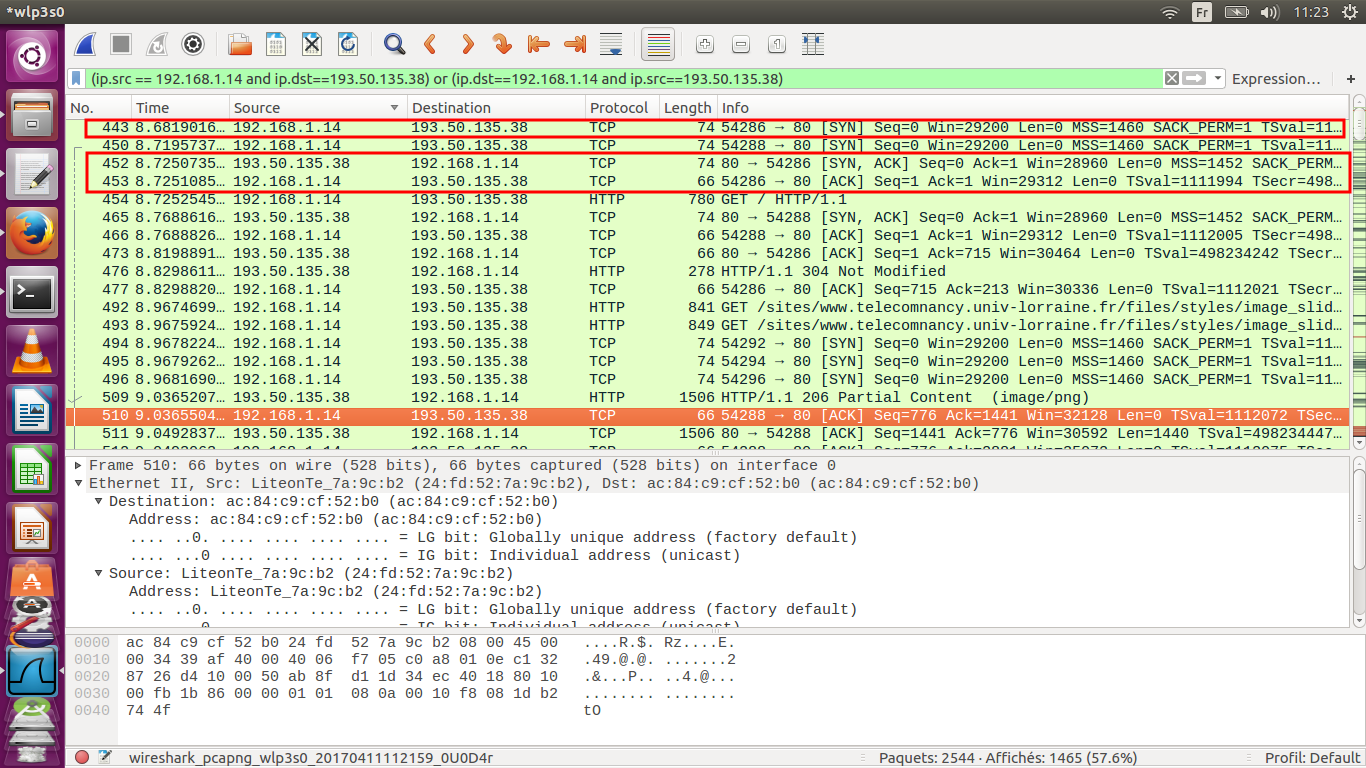
\includegraphics[scale=0.38]{Images/Connexion.png}
\end{figure}

\begin{figure}[p]
   \caption{\label{étiquette} Echanges}
   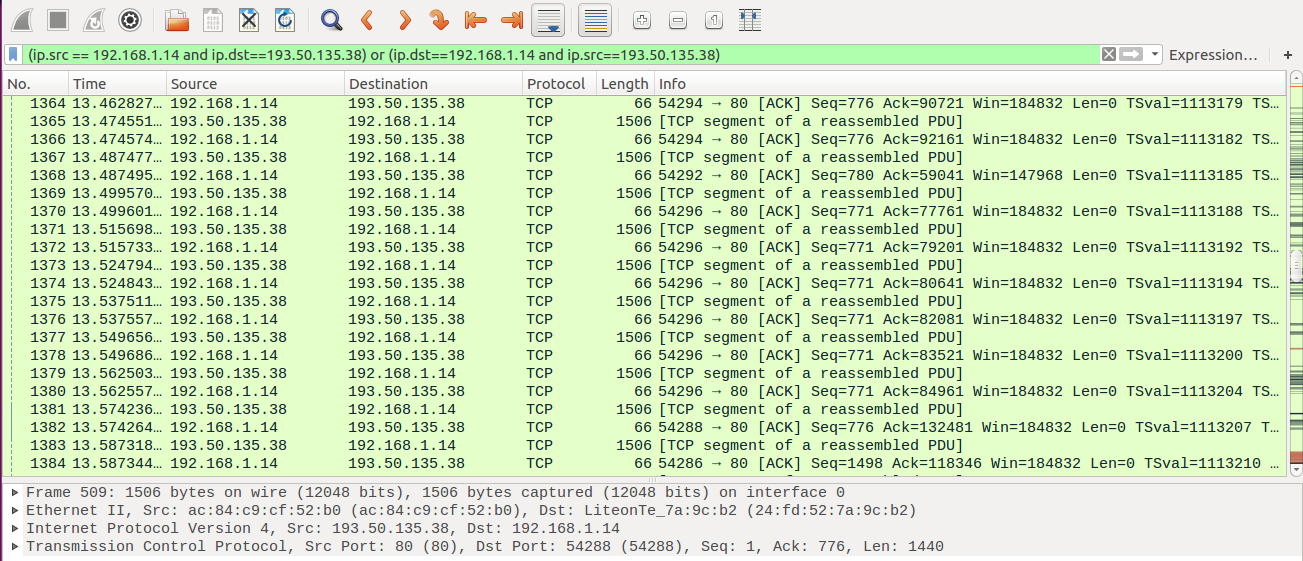
\includegraphics[scale=0.38]{Images/Echange.png}
\end{figure}


\newpage

\section*{\hspace{0.6cm}1.3\hspace{0.6cm}Avec proxy}

\hspace{1cm}Avec le proxy, la connexion fonctionne de la même façon qu'au dessus, sauf que les échanges se font entre notre machine et le proxy qui relaye les informations, et non directement avec le site web. Nous nous sommes connectés sur le réseau de l'école pour cette capture d'écran, ainsi notre adresse ip est: 10.10.98.98 et l'adresse du proxy utilisé est: 51.255.166.82 (une machine OVH personelle).\\

\begin{figure}[h]
   \caption{\label{étiquette} Avec Proxy}
   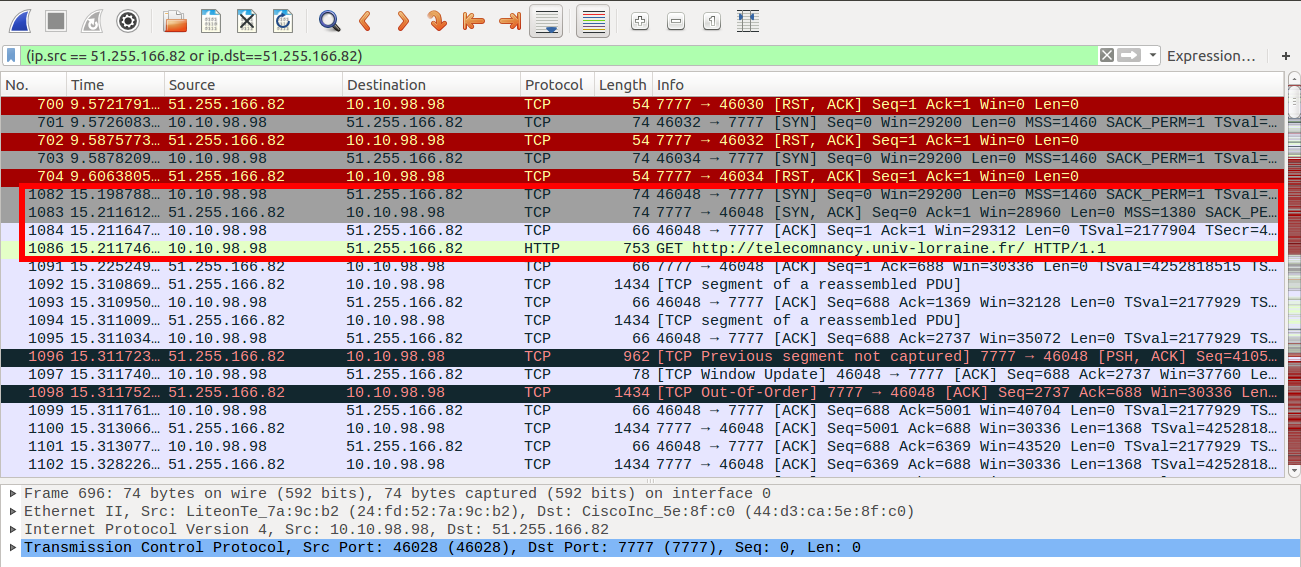
\includegraphics[scale=0.38]{Images/Proxy.png}
\end{figure}




\chapter*{2\hspace{1cm}Conception}

\section*{\hspace{0.6cm}2.1\hspace{0.6cm}Algorithme général gérant un client à la fois}

\begin{algorithm}[H]
 \KwData{Numéro de Port}\
 
 Creation du Serveur Proxy\;\
 
 \While{Vrai}{\
 
  Reception Connection Client\;\
  
  Recuperer Informations du message\;\
  
  \eIf{Message n'est pas une publicité}{\
  
   Envoyer Message au Serveur Web\;\
   
   Reception du Message du serveur du Serveur Web\;\
   
   Envoi du Message au Client\;\
   
   }\
   
 }
 \caption{Algorithme simple MyAdBlock}
\end{algorithm}

\newpage

\section*{\hspace{0.6cm}2.2\hspace{0.6cm}Précisions sur l'algorithme}
\hspace{1cm}La partie "Recupérer Information du message" comprend une récupération de la requête (\textit{GET}, \textit{CONNECT}...) et une récupération de l'adresse du serveur à contacter. Cette dernière récupération est implémentée telle que:\\

\lstset{language=C}

\renewcommand{\lstlistingname}{Algorithme}
\begin{lstlisting}[caption=Algorithme de détermination d'adresse serveur à contacter (messages.c)]

//Extrait hostname de "fromClient" et le met dans "host"
void getHost(char fromClient[], char host[]){
	int i=0;
	int j=0;
	char hostSearch[7] = "";

	//On passe jusqu'a ce qu'on arrive a "Host: "
	while(strcmp(hostSearch,"Host: ")!=0){
		for(j=0;j<6;j++){
			hostSearch[j] = fromClient[i+j];
		}
		hostSearch[6]='\0';
		i++;
	}
	
	//On saute le 2eme '/'
	i=i+5;
	j=0;
	//On recupere le nom jusqu'au prochain '/'
	while(fromClient[i] != '\n'){
		host[j] = fromClient[i];
		i++;
		j++;
	}
	host[j-1]='\0';
}

\end{lstlisting}

\newpage


\section*{\hspace{0.6cm}2.3\hspace{0.6cm}Implantation du multi-clients et passage Ipv4/Ipv6}
\hspace{1cm} Comme vu au TD2, nous avons utilisé la méthode \textit{SELECT()} pour éviter l'utilisation du multiprocessing ("fork" de serveurs) ce qui a permis de gérer les connexions multiples et simultanées. La primitive \textit{getaddrinfo()} nous permet d'avoir une socket d'écoute pour IPv4 et une autre pour IPv6. L'IPv6 coté client du proxy est également géré dans \textit{socket.c}\\

\lstset{language=C}

\renewcommand{\lstlistingname}{Algorithme}
\begin{lstlisting}[caption=Algorithme de gestion multi-clients et gestion IPv4/IPv6 (myAdBlock.c)]
for(;;){
	//Initialisation des fd_set puis SELECT
	pset=rset;
	nbfd=select(maxfdp1,&pset,NULL,NULL,NULL);
	if (nbfd==-1) {erreur...}
	
	// si connexion client
	if( FD_ISSET(server[0], &pset) || FD_ISSET(server[1], &pset) ){
		i = placelibre(tab_ecoute_clients);
		
		// si c'est en ipv4
		if( FD_ISSET(server[0], &pset) ){
			tab_ecoute_clients[i] = newCommunicationSock(server[0]);
		}
		
		// si c'est en ipv6 
		if( FD_ISSET(server[1], &pset) ){	
			tab_ecoute_clients[i] = newCommunicationSock(server[1]);
		}
		
		// mise a jour des variables
		FD_SET(tab_ecoute_clients[i], &rset);
		maxfdp1 = MaJ_maxFD(tab_ecoute_clients[i],maxfdp1);
		nbfd--;
	}
	
	i=0;
	//Parcours des tableau des clients et serveurs connectes
	while((nbfd>0)&&(i<FD_SETSIZE)){
		
		// on regarde si on a une reponse du serveur
		if(tab_ecoute_servers[i] >= 0 
		&& FD_ISSET(tab_ecoute_servers[i], &pset)){
			messageDuServeur(...);
			nbfd--;
		}
		// on regarde si on a une requete du client
		if(tab_ecoute_clients[i] >= 0 
		&& FD_ISSET(tab_ecoute_clients[i], &pset)){
			maxfdp1 = messageDuClient(...);
			nbfd--;
		}
		i++;
	}
}
\end{lstlisting}

\newpage
\section*{\hspace{0.6cm}2.4\hspace{0.6cm}Principe d'exclusion des publicités}

\hspace{1cm}Le code source de \textit{myAdBlock} ainsi que la liste \textit{MyAdListLight} des hosts de publicités sont dans le dossier \textit{src/}. Libre à vous d'ajouter des hosts dans la liste. \\

\hspace{0.40cm}Cette liste est une version allégée et plus simple de la liste de  \MYhref{https://easylist.to}{EasyList}, qui constitue notre banque de base de hosts de publicités. Voir  \MYhref{https://easylist.to/easylist/easylist.txt}{EasyList pour AdBlock Plus 2.0} pour consulter la banque complète. Chaque connexion entrante est filtrée, parsée et comparée à cette liste. Si elle appartient à cette liste, cette connexion est simplement bloquée (il s'agit d'une publicité). Compte tenu du fait que notre liste est réduite et ne tient pas comtpe des expressions régulières de la liste originale, myAdBlock est donc moins efficace que AdBlock (utilisant la même banque), mais est beaucoup plus simple et léger; et il est plus simple d'appréhender on fonctionnement. \\

\hspace{0.40cm}On remarque par ailleurs que notre 'bloqueur', ou plutôt comparateur, se matérialise par l'appel à \textit{contains()} de \textit{util.c}. Il consiste à vérifier que chaque token de notre liste \textit{MyEasyListLight} n'est pas contenu dans l'URL de la connexion entrante (voir Algorithme 3 et 4).\\

\renewcommand{\lstlistingname}{Algorithme}
\begin{lstlisting}[caption=Fonction contains() (util.c)]
bool contains(char URL[]){
	int i;
	for(i=0;i<sizeList;i++){
		if(strstr(URL, MyAdList[i])!=NULL){
			return true;
		}
	}
	return false;
}
\end{lstlisting}

\renewcommand{\lstlistingname}{Algorithme}
\begin{lstlisting}[caption=Fonction iniListe() qui charge la liste MyAdListLight(util.c)]
void iniListe() {
        FILE * fp; char * line = NULL; size_t len = 0; ssize_t read; int i=0;

        fp = fopen("src/MyAdListLight", "r");
        if (fp == NULL)	exit(EXIT_FAILURE);
	
	// on compte le nb de ligne
	while ((read = getline(&line, &len, fp)) != -1) { i++; }
	
	MyAdList = malloc(i*sizeof(char*));
	sizeList=i; 

	// on se remet le debut du fichier
	fseek(fp, 0, SEEK_SET); i=0;

	while ((read = getline(&line, &len, fp)) != -1) {
		MyAdList[i]=malloc(read*sizeof(char));
		strncpy(MyAdList[i],line,read-1);
		i++;	
	}
        fclose(fp);
}
\end{lstlisting}



\newpage
\hypersetup{linkcolor=blue}
\section*{\hspace{0.6cm}2.5\hspace{0.6cm}Extension du proxy : HTTPS}
\hspace{1cm} Pour gérer les connexions HTTPS entrantes, nous avons utilisé la méthode \textit{CONNECT}, permettant d'établir un tunnel sans déchiffrement. Une fois captée, la connexion HTTPS est filtrée comme une connexion HTTP standard. On peut le voir dans l'algorithme ci-dessous.\\

\renewcommand{\lstlistingname}{Algorithme}
\begin{lstlisting}[caption=Partie gérant l'HTTPS issue du CONNECT.]

else if(strcmp(typeRequete, "CONNECT") == 0){
			
	// On recupere le hostname du client
	getHost(fromClient,host);
	host[strlen(host)-4]='\0';
	
	if(contains(host)==false){
		// on cree le client sur le port d'ecoute 443
		tab_servers[i] = newClient(host,"443");

		//Mise a jour variables
		FD_SET(tab_servers[i], rset);
		maxfdp1 = MaJ_maxFD(tab_servers[i],maxfdp1);
		
		// on repond au client (accept): 
		// "HTTP/1.0 200 Connection established";
  		send(tab_clients[i],buffConnectionEstablished,
  		 strlen(buffConnectionEstablished), 0);
	}
	// si c'est une pub
	else {
		printf(" bloque :");
			send(tab_clients[i], buffOK, strlen(buffOK), 0);
		close(tab_clients[i]);
		FD_CLR(tab_clients[i], rset);
		tab_clients[i] = -1;
	}

	printf(" %s  %s\n",typeRequete,host);
}

\end{lstlisting}


\chapter*{3\hspace{1cm}Bibliographie}

\hspace{0.6cm}

\url{http://livre.g6.asso.fr/index.php/Exemple_de_client/serveur_TCP}

\url{http://livre.g6.asso.fr/index.php/Programmation_d'applications_bis}

\url{https://adblockplus.org/filter-cheatsheet}

\url{http://manpagesfr.free.fr/man/man3/getaddrinfo.3.html}

\url{https://fr.wikipedia.org/wiki/Hypertext_Transfer_Protocol}

\url{https://en.wikipedia.org/wiki/HTTPS}

\url{https://en.wikipedia.org/wiki/Transport_Layer_Security}


\end{document}